\section{Photonik Anwendungen}
\subsection{Lichtschranken}
\begin{multicols}{3}
    \subsubsection{Einweg-Lichtschranke}
    \begin{compactitem}
        \item Sender und Empfänger stehen sich gegenüber
        \item 1 Modul: Gabellichtschranke (z.B.: Drehzahlmesser)
        \item Sender und Empfänger getrennt: Justierung nötig
        \item Detektiert Unterbruch
    \end{compactitem}
    
    \subsubsection{Reflex-Lichtschranke}
    \begin{compactitem}
        \item Sender und Empfänger im selben Gehäuse: nur ein Kabel nötig
        \item Am anderen Ende Reflexfolie / Retroreflektor (Katzenauge)
        \item Detektiert Unterbruch
    \end{compactitem}
    
    \subsubsection{Reflex-Lichttaster}
    \begin{compactitem}
        \item Kein Reflektor: Normalerweise kommt kein Licht zurück
        \item Nahes Objekt reflektiert genügend Licht: Detektion
        \item Von Objekteigenschaften abhängig!
    \end{compactitem}
\end{multicols}

\subsubsection{Nachteile}
\begin{compactitem}
    \item Fremdlicht kann die Funktion der Lichtschranke beeinflussen
    \item Möglichkeiten der Unterdrückung
    \begin{compactitem}
        \item Optischer Filter: nur das Licht, dass ausgesandt wird, gelangt zum Detektor, Fremdlicht mit anderem Spektrum wird unterdrückt
        \item Mehr Leistung: Optik, LED zu Laser, Verhältnis Nutz- zu Fremdlicht verbessert sich
        \item Moduliertes Licht: Mit elektrischem Filter wird die Modulationsfrequenz herausgesucht
    \end{compactitem}
\end{compactitem}

\begin{multicols}{2}
    \subsection{Ambientlight Sensor (ALS)}
    \begin{compactitem}
        \item Detektiert die Umgebungshelligkeit zum Dimmen des Displays
        \item Ist oftmals eine Photodiode
        \item Meist im Proximity-Sensor eingebaut
        \item Teils mit RGB-Farbdetektion
    \end{compactitem}
    
    \subsection{Proximity-Sensor}
    \begin{compactitem}
        \item kleiner Reflexlichttaster
        \item Unterschiedliche Reflexion von heller/dunkler Haut und blondem/schwarzem Haar sowie Schmutz auf dem Glas können Probleme verursachen.
    \end{compactitem}
\end{multicols}

\subsection{Optische Distanzmessung}
\subsubsection{Vergleich}
\begin{multicols}{4}
    \paragraph{Stereo}
    \begin{compactitem}
        \item Passive Messung
        \item Objektstruktur nötig, Abschattungen möglich
        \item Rechenaufwändig
    \end{compactitem}
    
    \paragraph{Laufzeitmessung (Time-of-Flight)}
    \begin{compactitem}
        \item Aktive Beleuchtung nötig
        \item Keine Abschattung
    \end{compactitem}
    \ \\
    
    \paragraph{Triangulation}
    \begin{compactitem}
        \item Aktive Beleuchtung nötig
        \item Keine Struktur nötig
        \item Relativ einfache Berechnung
    \end{compactitem}
    \ \\
    
    \paragraph{Interferometrie}
    \begin{compactitem}
        \item Höchste Auflösung
        \item Aufwändige Technik
    \end{compactitem}
    \ \\ \ \\ \ \\
\end{multicols}

\newpage
\subsubsection{Stereo Messung}
\begin{wrapfigure}[6]{l}{0.3\textwidth}
    %\vspace{-12pt}
    \centering
    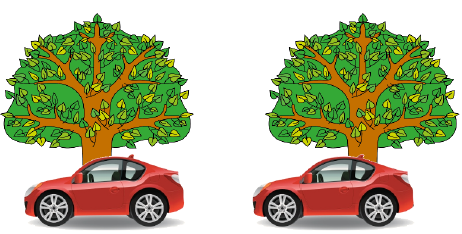
\includegraphics[width=0.25\textwidth]{images/photonik_anwendung_stereo}
\end{wrapfigure}
\ 
\vspace{-5pt}
\begin{compactitem}
    \item Diese Methode ist dem menschlichen Sehen nachempfunden.
    \item Es ist ein passives System: keine Beleuchtung nötig.
    \item Eine aufwändige Berechnung ist notwendig (Kreuzkorrelation zwischen den Bildern muss berechnet werden).
    \item Einfarbige Flächen können nicht bestimmt werden.
\end{compactitem}

\subsubsection{Triangulations Messung}
\begin{wrapfigure}[4]{l}{0.3\textwidth}
    %\vspace{-12pt}
    \centering
    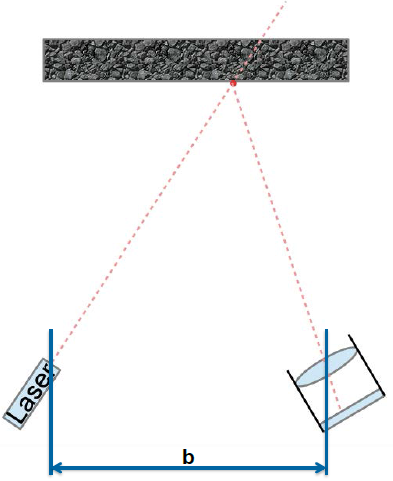
\includegraphics[width=0.1\textwidth, angle=90]{images/photonik_anwendung_triangulation}
\end{wrapfigure}
\ 
\vspace{-5pt}
\begin{compactitem}
    \item Ein Zeilensensor misst den Fokus des reflektierten Laserlichts.
    \item Mit der Winkelbeziehung wird die Distanz bestimmt.
    \item Eine Beleuchtung ist nötig.
    \item Einfache Detektion und Berechnung der Distanz über die Geometrie.
\end{compactitem}

\subsubsection{Time-of-Flight Messung}
\begin{compactitem}
    \item Ein perfekter Puls kann nicht generiert werden.
    \item Die Modulation einer Lichtquelle mit Sinussignal ist eine Alternative. 
    \item Es wird dann der Phasenunterschied vom ausgesendeten zu empfangenen Signal gemessen.
    \item Nachteil: Nicht ein-eindeutige Position, Auflösung nur innerhalb einer Periode möglich
\end{compactitem}

\paragraph{Funktionsweise}
\begin{wrapfigure}[4]{l}{0.3\textwidth}
    %\vspace{-12pt}
    \centering
    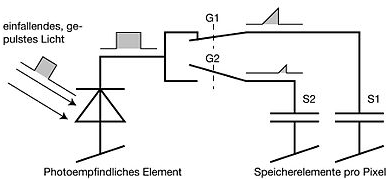
\includegraphics[width=0.29\textwidth]{images/tof_fkt_01}
    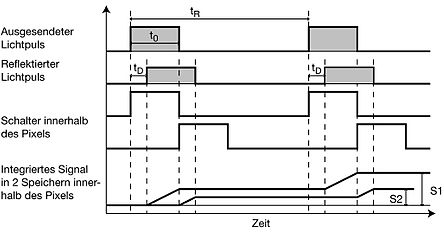
\includegraphics[width=0.29\textwidth]{images/tof_fkt_02}
\end{wrapfigure}
\ 
\vspace{-5pt}
\begin{compactenum}
    \item Puls-Signal wird ausgesendet.
    \item Licht des Sensors wird abwechselnd auf 2 Kapazitäten geschaltet
    \item Je nach Verzögerung ist die Verteilung der Photonen anders.
    \item Es liegen somit andere Spannungen an S1 und S2.
    \item Daraus kann ein Rückschluss auf Eintreff-Zeit des Pulses gemacht werden.
    \item Verschiebt sich die Ankunft des Pulses, so verändern sich Anteile die S1 und S2.
    \item Daraus kann die Distanz berechnet werden. \\
\end{compactenum}

\ \\
\subsection{Optische Datenübertragung}
\subsubsection{Vorteile}
\begin{compactitem}
    \item Licht anstelle eines elektrischen Signals als Übertragungsmedium
    \item Störungsarm: kein elektrisches Einkoppeln, kein Übersprechen, keine Potentialprobleme
    \item Kleine Dämpfung, grosse Reichweite
    \item Grosse Bandbreite: $>$ 100Gbit/s
\end{compactitem}

\subsubsection{Glasfaserarten}
\begin{wrapfigure}[14]{l}{0.6\textwidth}
    %\vspace{-12pt}
    \centering
    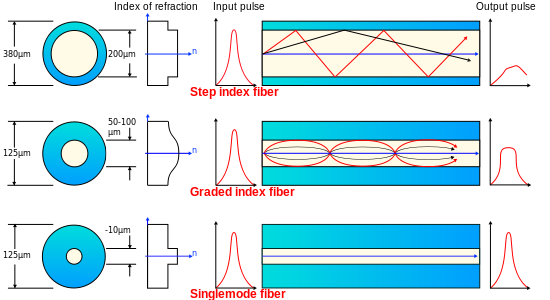
\includegraphics[width=0.55\textwidth]{images/glasfaserarten}
\end{wrapfigure}
\ 
\vspace{-5pt}
\begin{compactitem}
    \item POF: (polymericopticalfibre), Kunststoff, \\
    Ø = 1mm, billig, Kopplung an LED, \\
    kleine Datenrate $<$100MB/s, kurze Verbindung
    \item Multimode (Mantel orange, türkis), \\
    Ø = 50$\mu$m/62.5$\mu$m, \\
    hohe Datenrate
    \item Monomode(gelb), \\
    Ø $<$10$\mu$m, \\
    höchste Datenrate
\end{compactitem}
\ \\

\subsubsection{Glasfaser als Sensor}
\begin{multicols}{2}
    \paragraph{Faserkreisel}
    \begin{compactitem}
        \item Bei Ruhe: Lichtwege sind identisch, konstruktive Interferenz
        \item Bei Drehung: der eine Lichtweg wird etwas kürzer, der andere länger, destruktive Interferenz, resp. das Linienmuster verschiebt sich
    \end{compactitem}
    
    \paragraph{Faseroptische Druck-und Temperatursensoren}
    \begin{compactitem}
        \item Durch Druck oder Temperatur ändert sich die (Raman-) Reflexionan dieser Stelle, örtlich aufgelöste Messung
        \item Wird eingesetzt bei Staumauern, Flugzeugflügel, ...
        \item Einfacher Sensor, «aber teure Auswertung
    \end{compactitem}
\end{multicols}

\subsection{Kontaktlose Temperaturmessung mittels Infrarotstrahlung}
\subsubsection{Seebeck-Effekt}
\begin{compactitem}
    \item Der Seebeck-Effekt tritt auf bei Temperaturdifferenzen in Leitern.
    \item Am warmen Ende eines Leiters haben Elektronen mehr Energie als am kalten Ende.
    \item Die Beweglichkeit der Elektronen ist grösser.
    \item Durch Diffusion bewegen sich mehr energiereiche Elektronen zum kalten Ende als energiearme Elektronen in die entgegengesetzte Richtung.
    \item Durch diese Thermodiffusionsströme entsteht zwischen den Kontaktstellen eine elektrische Spannung, die Thermo- oder Seebeck-Spannung.
\end{compactitem}


\begin{minipage}{0.45\textwidth}
       \begin{equation*} 
        \begin{split} 
          &V_{out}=N \cdot S \cdot(T_x - T_{REF})\\
          &\text{N: Number of thermocouples}\\
          &\text{S: Seebeck coefficient}
        \end{split} 
      \end{equation*}

\end{minipage}
\begin{minipage}{0.5\textwidth} 
    \vspace{-0.5cm}
    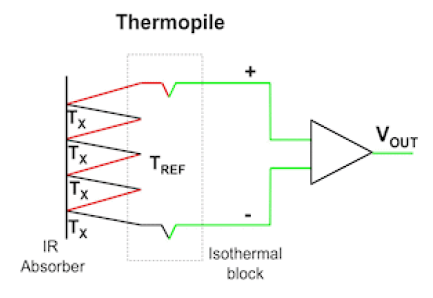
\includegraphics[width=1\textwidth]{images/Thermo}
\end{minipage}

